\section{Цель работы}
Цель работы --- решить задачу Коши для обыкновенных
дифференциальных уравнений численными методами.

\section{Рабочие формулы}
\begin{itemize}
\item Метод Эйлера
  \[ y_{i+1} = y_i + h y'(x_i, y_i) \]
\item Метод Рунге-Кутта 4-го порядка
  \[ y_{i+1} = y_i + 1/6 (k_1 + k_2 + k_3 + k_4) \]
  \(k_1 = h f(x_i, y_i)\), \(k_2 = h f (x_i + h/2, y_i + k_1 / 2 )\),
  \( k_3 = h f(x_i + h/2, y_i + k_2 / 2) \),
  \( k_4 = h f(x_i + h, y_i + k_3) \).
\item Метод Милна
  \begin{align*}
    y_i^\text{прогн} &= y_{i-4} + 4/3 h ( 2 f_{i-3} - f{i-2} + 2 f_{i-1} ) \\
    y_i^\text{корр}  &= y_{i-2} + h/3 (f_{i-2} 4 f_{i-1} f_i^\text{прогн}) \\
    f_i^\text{прогн} &= f(x_i, y_i^\text{прогн})
  \end{align*}
\end{itemize}

\section{Исходный код}
\inputminted[breaklines]{python}{../main.py}

\section{Результаты работы}
\begin{center}
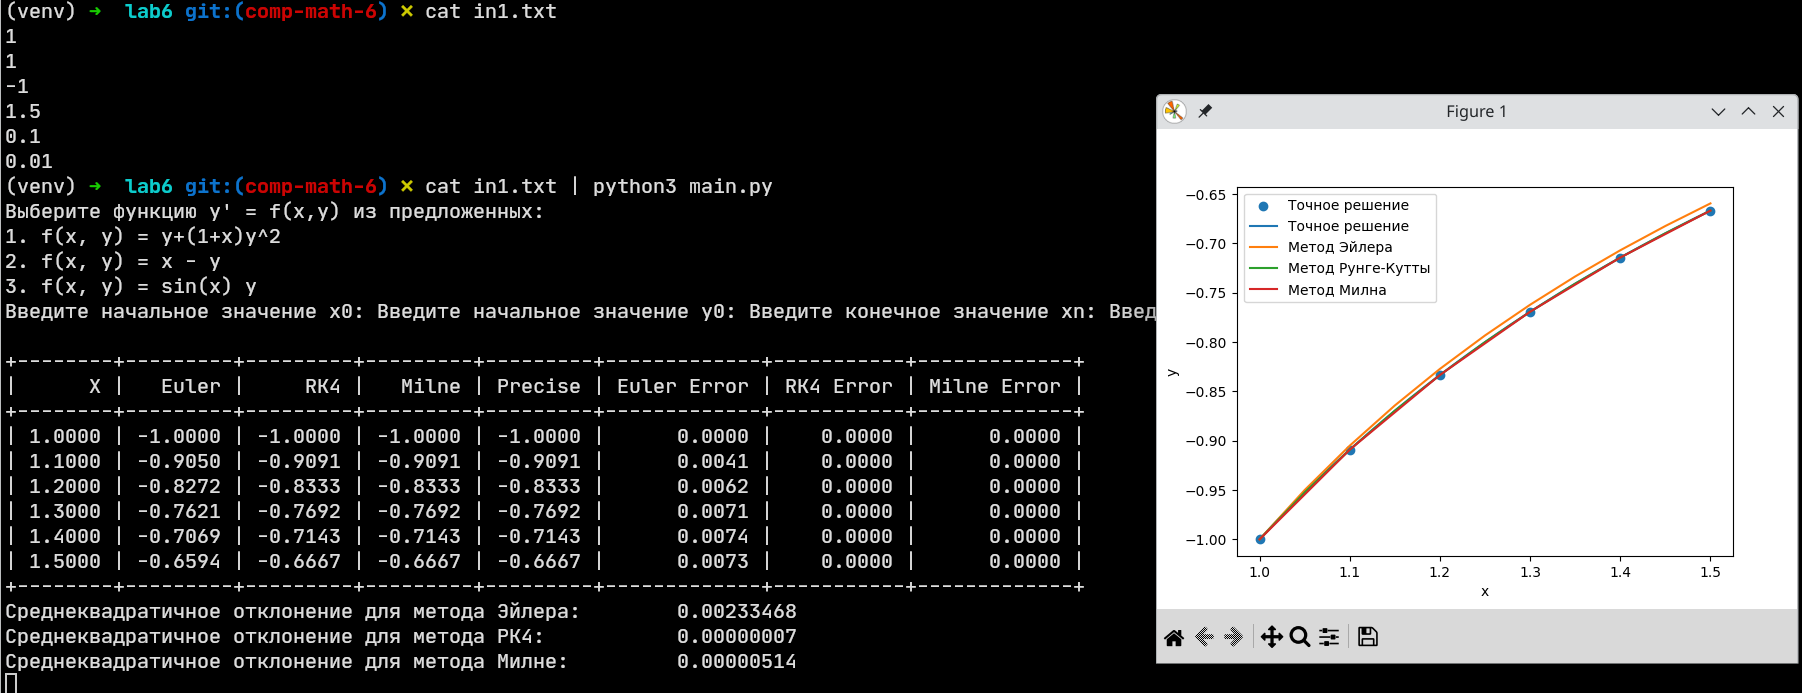
\includegraphics[width=\textwidth]{./img/demo1.png}
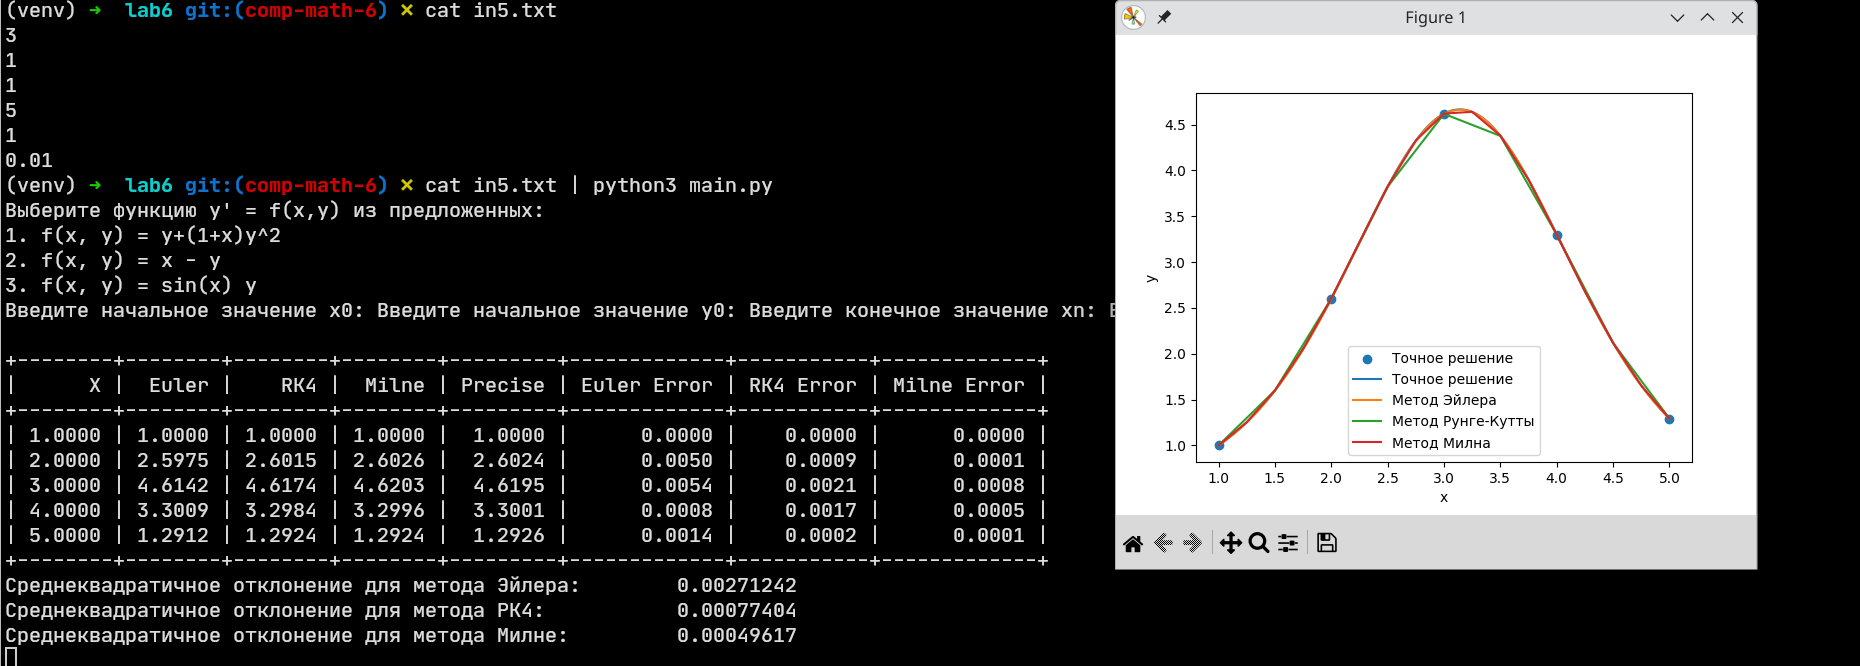
\includegraphics[width=\textwidth]{./img/demo2.png}
\end{center}

\section{Вывод}
В ходе выполнения данной лабораторной работы мною были изучены
методы решения обыкновенных дифференциальных уравнений, такие как
метод Эйлера, метод Рунге-Кутта и метод Милна. Эти методы
были реализованы мной на языке программирования Python 
и проверены при разных функциях и входных параметрах.
